\section{Implementation Overview}
% Describe the design of your program. Justify the decisions you made.
The simulator implements several predictors that can be run for a given trace file. An overview of each predictor is given in Figure \ref{fig:predictors}. The one-bit, two-bit and global predictors were developed using material from lectures. The GShare predictor was developed using online resources as a guide on the concept, including the original GShare paper \cite{gshare_paper}, a lecture on branch prediction \cite{pittsburg_branch_prediction}, another university assignment \cite{gshare_assignment_edinburgh} and documentation for the Berkeley Out-of-Order Machine's branch prediction \cite{gshare_boom_core}. Running the simulator without a specified trace file will run all trace files in the \texttt{trace-files} folder. Each trace file is run with all possible predictor types and table sizes. After running one configuration, the table size and misprediction rate is exported into a \texttt{csv} file for the trace file and predictor type. These files served as graph data for the graphs in this report.

\begin{figure}[H]
    \begin{framed}
        \begin{itemize}
            \item Always Taken: Always predicts a branch to be taken.
            \item One-Bit: Keeps a table of booleans used to predict the outcome of a branch. The program counter address space maps directly to the table.
            \item Two-Bit: Keeps a table of integers used to predict the outcome of a branch. The integer is set from 0 to 3 to represent FSM states (strongly not taken, weakly not taken, weakly taken and strongly taken). The program counter address space maps directly to the table. A diagram of the FSM is shown in Figure \ref{fig:twoBitPredictorImage}.
            \item Global: Uses a bit predictor for each possible outcome of previous branches (taken or not taken). Whether to use one-bit or two-bit predictors is set at initialisation. The outcomes are tracked using a boolean value. This value is used to choose the predictor.
            \item GShare: Uses a long as a global history register for branch outcomes. This is XORed with the program counter address to map into a two-bit predictor table. Bit shifting and setting enable each bit of the long to represent a previous outcome. A diagram is shown in Figure \ref{fig:gShareImage}.
            \item Profiled: Looks at the outcome of each conditional branch in advance and then chooses to take it if it was taken more than it was not taken.
        \end{itemize}
    \end{framed}
    \caption{A textual overview of predictor types implemented}
    \label{fig:predictors}
\end{figure}

\begin{figure}[htbp]
    \centering
    \subfigure[Overview of a two-bit predictor's finite-state machine for a table entry \cite{gshare_boom_core}]{
    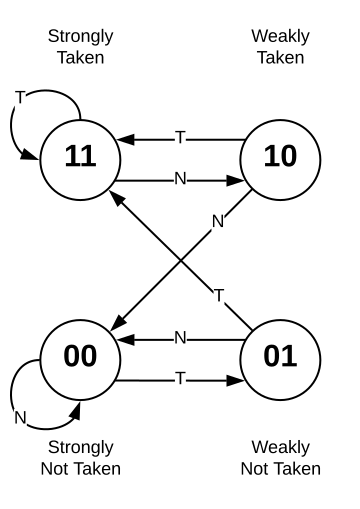
\includegraphics[width=0.425\textwidth, height=0.3\textheight, keepaspectratio]{Images/2BitPredictor.png}
        \label{fig:twoBitPredictorImage}
    }
    \hfill
    \subfigure[Overview of a GShare predictor, showing XOR mapping into a two-bit predictor table \cite{gshare_boom_core}]{
        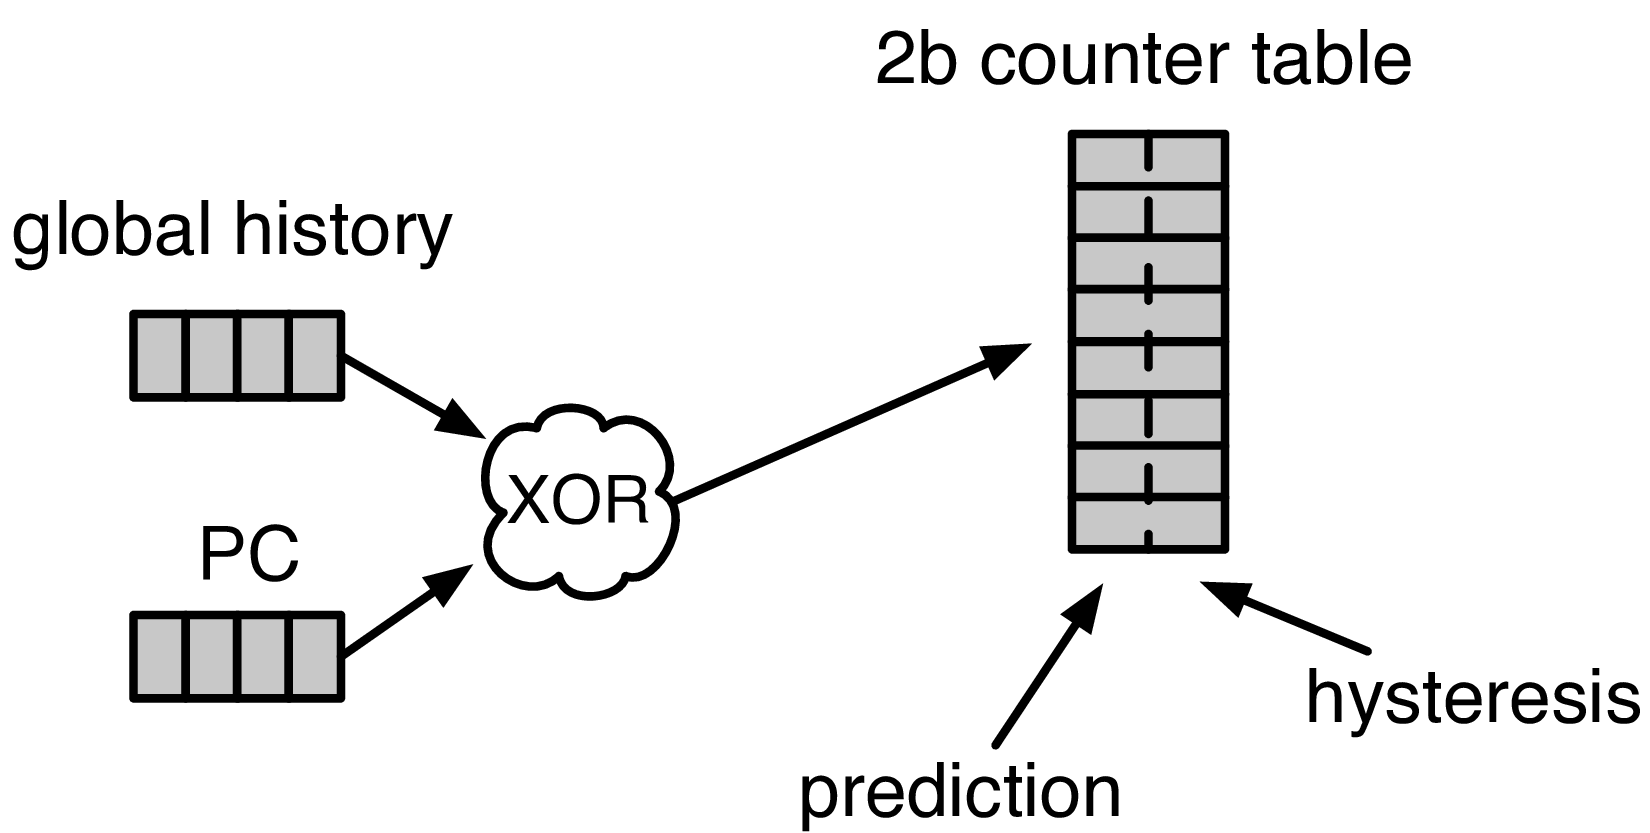
\includegraphics[width=0.525\textwidth, height=0.3\textheight, keepaspectratio]{Images/GSharePredictor.png}
        \label{fig:gShareImage}
    }
    \caption{A visual overview of predictor concepts}
    \label{fig:predictorImages}
\end{figure}
